\documentclass[aspectratio=169]{beamer}
\usetheme{Madrid}
\usecolortheme{seahorse}
\usepackage{booktabs}
\setbeamertemplate{navigation symbols}{}

\newcommand{\todo}[1]{{\color{red}\textbf{[TODO: #1]}}}

\title[Over-Squashing vs.\ Robustness]{Over-Squashing \emph{vs.}\ Adversarial Robustness in GNNs}
\subtitle{An ``Add \emph{vs.}\ Remove Edge'' Investigation}
\author[Kompayak, Niamsa-Ard]{Supanut Kompayak (st126055) \and Dechathon Niamsa-Ard (st126235)}
\institute[AIT]{Deep Learning Course Project, Asian Institute of Technology}
\date{7 July 2026}

\begin{document}

\frame{\titlepage}

\begin{frame}{The question}
  Two GNN problems that look unrelated, but both are about \textbf{structural sensitivity}:
  \begin{itemize}
    \item \textbf{Over-squashing} --- long-range signal squeezed through bottlenecks and lost.
      Output \emph{not sensitive enough} to distant nodes.
    \item \textbf{Adversarial fragility} --- a few edited edges flip the prediction.
      Output \emph{too sensitive} to malicious structural change.
  \end{itemize}
  \vfill
  \centering\Large Do methods that fix over-squashing also help robustness?
\end{frame}

\begin{frame}{The spine: add \emph{vs.}\ remove edge}
  \begin{itemize}
    \item Over-squashing rewiring: FoSR \textbf{adds} edges; spectral pruning \textbf{removes} edges
      (both raise the spectral gap).
    \item Adversarial attack: \textbf{adds} dissimilar edges. Defense (GCN-Jaccard): \textbf{removes} them.
  \end{itemize}
  \vfill
  Hypothesis: \emph{adding} to fix over-squashing may \emph{hurt} robustness (more edges to exploit);
  \emph{removing} for over-squashing may \emph{transfer} to robustness (removes like a defense).
\end{frame}

\begin{frame}{Methods (the design)}
  \centering
  \begin{tabular}{@{}llll@{}}
    \toprule
    Method & Targets & Edge op & Role \\
    \midrule
    GCN (vanilla)        & ---            & none   & baseline \\
    FoSR                 & over-squashing & add    & ``add'' arm \\
    ProxyDelete          & over-squashing & remove & ``remove'' arm \\
    GCN-Jaccard          & defense        & remove & defense reference \\
    DropEdge             & regularization & random & random-removal control \\
    \bottomrule
  \end{tabular}
  \vfill
  \footnotesize FoSR vs.\ ProxyDelete = direction; ProxyDelete vs.\ Jaccard = criterion.
\end{frame}

\begin{frame}{Setup}
  \begin{itemize}
    \item \textbf{Cora \& Citeseer} node classification, DeepRobust \texttt{nettack} split, CPU.
    \item Attack: Metattack (poisoning), ptb $\{0.05, 0.10\}$; cached once, reused.
    \item Pipeline: \texttt{clean} $\to$ Metattack $\to$ method $\to$ train GCN $\to$ eval.
    \item Metric: clean / robust accuracy, robustness \textbf{gap} $=$ clean $-$ robust.
  \end{itemize}
  \vfill
  \centering
  \begin{tabular}{@{}lccc@{}}
    \toprule
    \textbf{Dataset} & \textbf{Nodes}$^{\ast}$ & \textbf{Classes} & \textbf{Features} \\
    \midrule
    Cora     & 2{,}485 & 7 & 1{,}433 \\
    Citeseer & 2{,}110 & 6 & 3{,}703 \\
    \bottomrule
  \end{tabular}\\[3pt]
  {\footnotesize $^{\ast}$standard \texttt{nettack} split (largest connected component)}
\end{frame}

\begin{frame}{Results: add vs.\ remove under attack (Cora)}
  \centering
  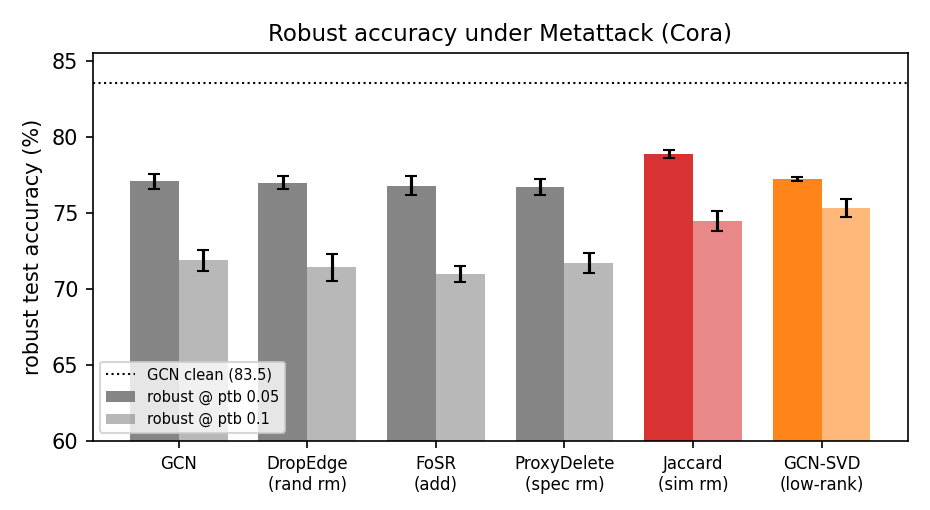
\includegraphics[height=0.6\textheight]{figures/headline.png}
  \vfill
  \footnotesize Four arms (GCN, DropEdge, FoSR, ProxyDelete) cluster at the GCN level; \textbf{the two
  purpose-built defenses separate} --- Jaccard (similarity) \& SVD (low-rank). The add/remove
  \emph{direction} does not matter --- the editing \emph{criterion} does.
\end{frame}

\begin{frame}{Why does Jaccard win? (mechanism)}
  Metattack almost purely \textbf{adds} edges (503 added, 3 removed at ptb 0.10). How many does each
  method delete?
  \vfill
  \centering
  \begin{tabular}{@{}lccc@{}}
    \toprule
    Method (ptb .10) & \# removed & attack edges rm. & recall \\
    \midrule
    \textbf{GCN-Jaccard}   & 797 & 250 & \textbf{0.50} \\
    ProxyDelete (spectral) & 643 & 93  & 0.19 \\
    DropEdge (random)      & 643 & 59  & 0.12 \\
    FoSR (add)             & 0   & 0   & 0.00 \\
    \bottomrule
  \end{tabular}
  \vfill
  \footnotesize Chance recall $\approx0.12$. Jaccard deletes \textbf{half} the attack edges
  ($\sim$4$\times$ chance) $\Rightarrow$ it undoes the attack. Spectral/random $\approx$ chance; add
  removes none.
\end{frame}

\begin{frame}{Over-squashing probe (RQ1)}
  \centering
  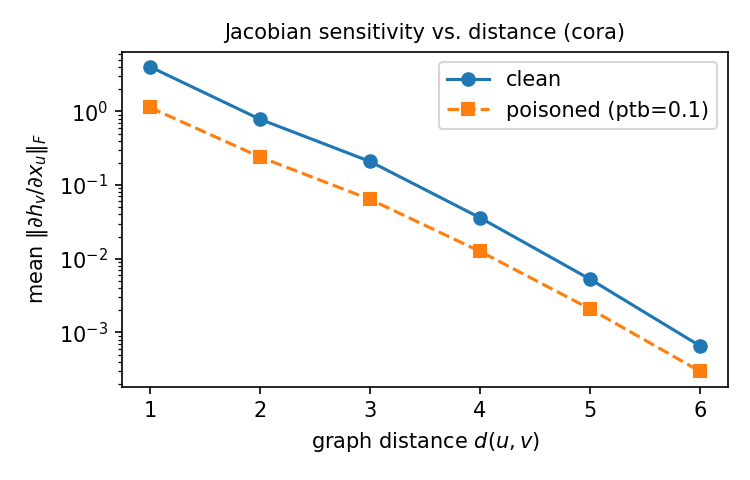
\includegraphics[height=0.6\textheight]{figures/probe.png}
  \vfill
  \footnotesize Sensitivity decays $\sim$5$\times$/hop $\Rightarrow$ over-squashing is real. Poisoning
  shifts the level but \textbf{not} the decay rate $\Rightarrow$ over-squashing \& fragility are
  decoupled (matches RQ2).
\end{frame}

\begin{frame}{Adaptive attacker: evadable but self-defeating}
  A Jaccard-aware attacker adds edges between feature-\textbf{similar} nodes (the filter won't remove them).
  \begin{itemize}
    \item Evasion works at the filter: Jaccard removes \textbf{0\%} of these edges.
    \item But the attack turns weak: GCN drops only $0.7$/$2.1$ pts (vs $6.5$/$11.7$ for Metattack).
    \item[$\Rightarrow$] Edges that fool the model (dissimilar) are the ones Jaccard removes; edges that
      evade Jaccard (similar) barely fool it --- \textbf{potency \& detectability are coupled}.
  \end{itemize}
  \footnotesize Heuristic (not gradient-optimal) adaptive attack; optimal adaptive $=$ future work.
\end{frame}

\begin{frame}{Findings: which knob decides robustness?}
  \vfill
  \centering
  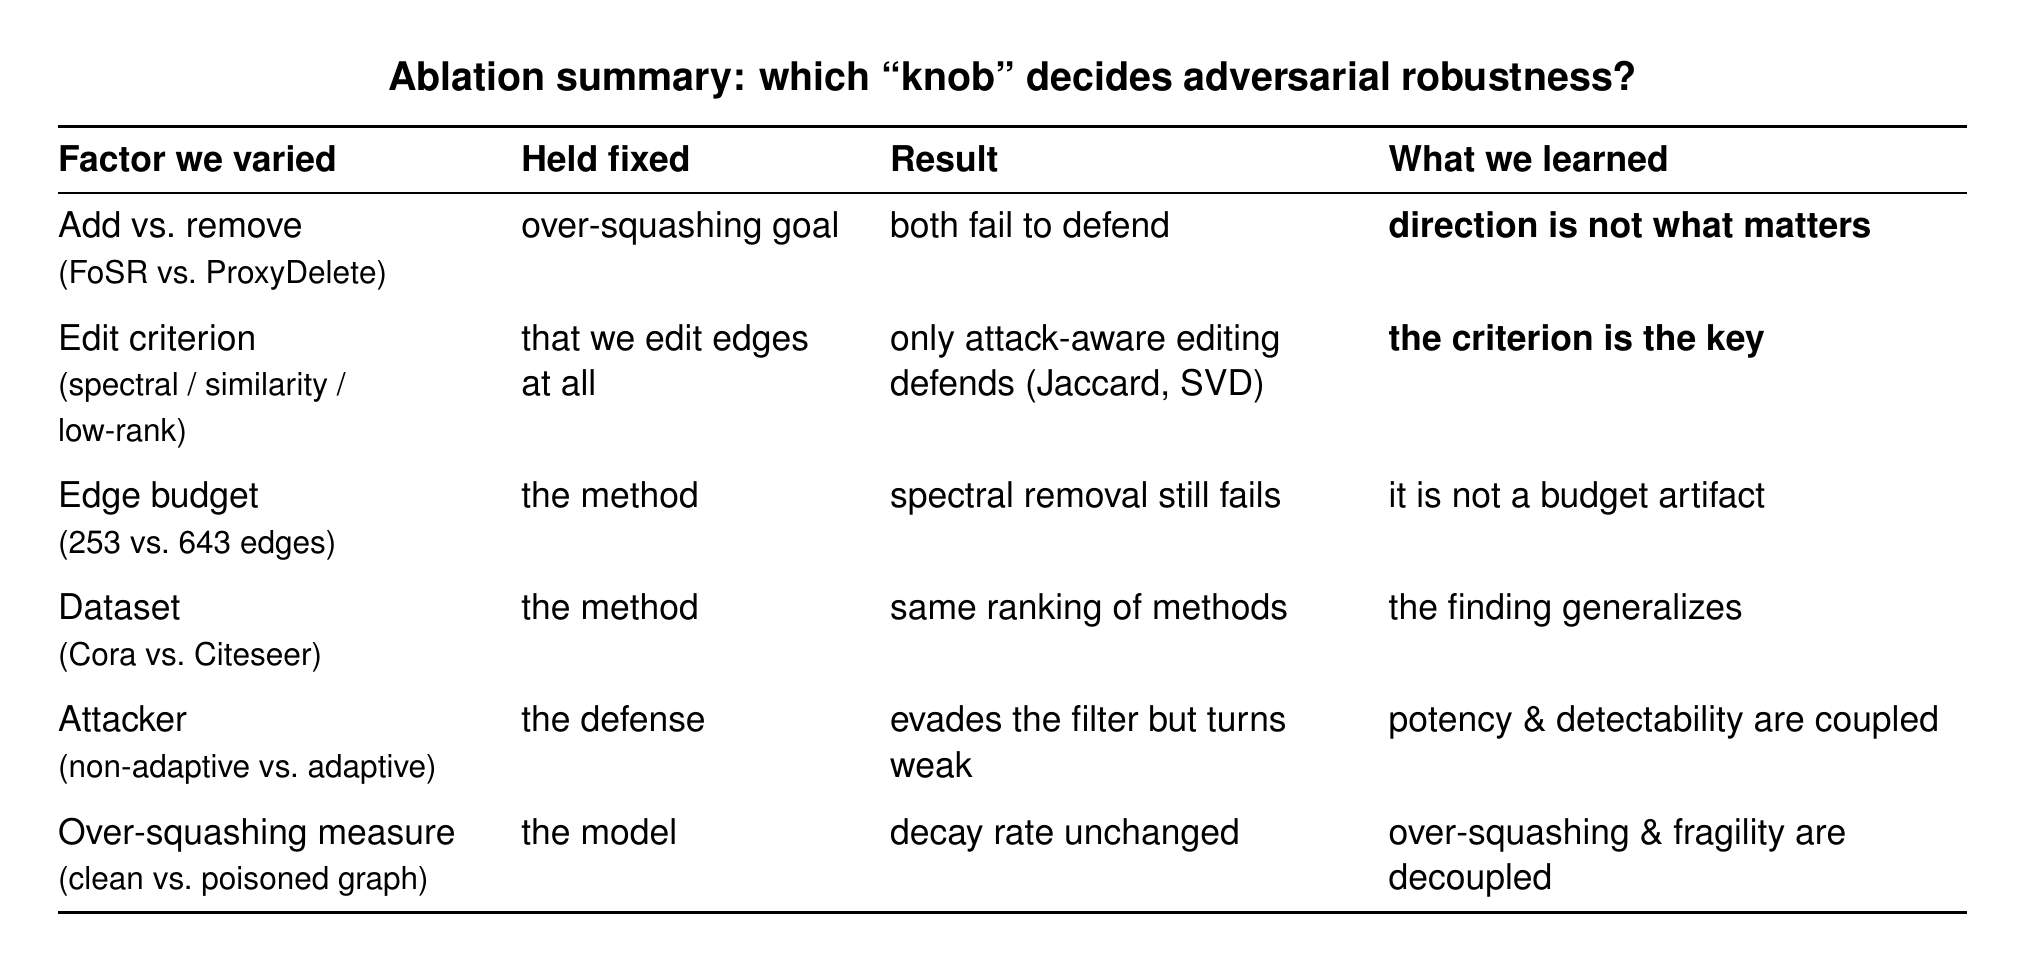
\includegraphics[width=0.97\textwidth]{figures/ablation_summary.png}
  \vfill
\end{frame}

\begin{frame}{Conclusion}
  \begin{itemize}
    \item Over-squashing mitigations (FoSR add, ProxyDelete spectral-remove) \textbf{do not} improve
      adversarial robustness on Cora / Metattack.
    \item Only attack-aware defenses defend --- Jaccard (similarity) \& SVD (low-rank); robustness comes
      from targeting the attacker's edges, not from optimizing the spectral gap.
    \item Honest negative result: the over-squashing $\to$ robustness bridge is \emph{not} supported here.
    \item Robust to budget (spectral removal still fails at 643 edges) \& replicated on
      \textbf{Cora + Citeseer}. A defense-aware attacker evades Jaccard only by turning weak.
    \item Next: gradient-optimal adaptive attack, RQ3 (Jacobian $\to$ fragility).
  \end{itemize}
\end{frame}

\begin{frame}{}
  \centering \Huge Thank you \\[1em] \normalsize Questions?
\end{frame}

\end{document}
